\section{APL}

\begin{frame}[fragile]{Kenneth E. Iverson}

    \begin{figure}
        \centering 
        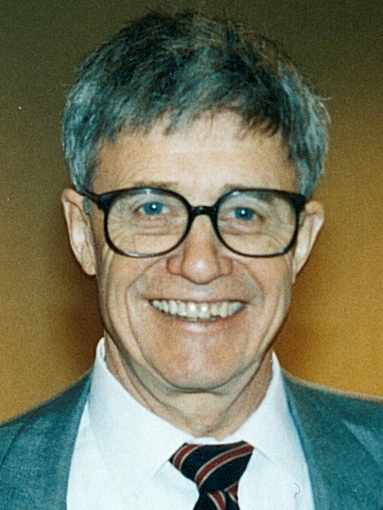
\includegraphics[scale=1.2]{figs/iverson.png}
        \caption{Kenneth Eugene Iverson (\gtrsymBorn 1920 -- \gtrsymDied 2004)}
    \end{figure}

\end{frame}

\begin{frame}[fragile]{Iverson e a notação matemática}

    \begin{itemize}
        \item Ao longo de sua carreira acadêmica, Iverson sempre esteve especialmente interessado na notação matemática 
        \pause

        \item Ele achava a notação matemática inconsistente e imprecisa
        \pause

        \item Por exemplo, na matemática alguns operadores são pré-fixados, como o sinal de negativo ($-n$), e outros são pós-fixados, como no caso do fatorial ($n!$)
        \pause

        \item No caso do valor absoluto, o operando fica cercado por dois símbolos ($|n|$)
        \pause

        \item Algumas operações de fato nem tem símbolos associados, como a exponeciação, que anota o expoente como superescrito da base ($a^b$)
        \pause

        \item Além disso, as diferentes regras de precedência da matemática levam ao uso de parêntesis e ambiguidades (a expressão $a / bx$ significa $a / (bx)$ ou $(a/b)x$?)
    \end{itemize}

\end{frame}

\begin{frame}[fragile]{Criação da APL}

    \begin{itemize}
        \item Na percepção de Iverson, nem a notação matemática nem linguagens de programação como Fortran permitiam a expressão, publicação e discussão fluente de algoritmos 
        \pause

        \item Este pensamento o levou a desenvolver e propor uma nota notação em 1957, enquanto lecionava em Harvard
        \pause

        \item Posteriormente, enquanto trabalhava na IBM e desenvolvia sua nova notação, ele e seus colaboradores a chamavam \textit{Iverson's Better Math}

        \pause
        \item A empresa não gostou do trocadilho e o nome da notação mudou para \textit{A Programming Language} -- APL
        \pause

        \item Este nome foi usado oficialmente pela primeira vez em 1962, quando Iverson publicou o livro \textit{A Programming Language}
    \end{itemize}

\end{frame}

\begin{frame}[fragile]{APL -- A notação e a linguagem}

    \begin{itemize}
        \item A notação APL foi usada internamente na IBM na década de 60
        \pause

        \item A nova notação proposta por Iverson permitiria a escrita de programas de computador claros e concisos
        \pause

        \item Contudo, a proposta inicial, descrita no livro, não podia ser replicada ou inserida diretamente em um computador
        \pause

        \item Por meio do apoio de colaboradores, como Adin Falkoff, Iverson elaborou uma nova APL que poderia ser usada em sessões interativas em um computador
        \pause

        \item A linguagem APL é baseada na notação de Iverson, descrita no livro homônimo, e, embora diferente, mantém vários de seus conceitos fundamentais
    \end{itemize}

\end{frame}

\begin{frame}[fragile]{Desenvolvimentos iniciais da APL}

    \begin{itemize}
        \item Em 1962 foi feita a primeira tentativa de descrever um sistema computacional completo baseado em APL, motivada por uma discussão entre Fallkoff e o Dr. William C. Carter
        \pause

        \item No ano seguinte o Dr. Herbert Hellerman implementou parte da notação em um IBM 1620 e estudantes do ensino médio usaram esta implementação (PAT)
        \pause

        \item Ainda em 1963 Falkoff, Iverson e Edward H. Sussenguth Jr. trabalharam juntos em uma implementação da APL, visando o desenvolvimento de programação e uso de computadores na educação
        \pause

        \item No ano de 1965 Lawrence M. Breed e Philip S. Abrams implementaram uma parte da notação em FORTRAN IV (chamada IVSYS -- \textit{Iverson System})
        \pause

        \item Assim como no PAT, IVSYS ainda não usavam glifos para representar funções e operandos, mas palavras reservadas em inglês
    \end{itemize}

\end{frame}

\begin{frame}[fragile]{Evolução da APL}

    \begin{itemize}
        \item A evolução do APL passou, no ano de 1964, pelo desenvolvimento de hardwares capazes de inserir e imprimir os glifos
        \pause

        \item A primeira tentativa de uma sessão interativa de APL foi feita por Larry Breed em 1966
        \pause

        \item A IBM introduziu a APL no mercado em 1967, em um computador IBM 1130
        \pause

        \item Na década de 70 a APL era utilizada por pesquisadores da IBM, na NASA e em instituições financeiras
        \pause

        \item APL ganhou terreno nos \textit{mainframes} entre as décadas de 60 e 80
        \pause

        \item Em 1979, Iversion ganhou o Turing Award pelo seu trabalho na APL
        \pause

        \item Décadas depois, Iverson também inventou a linguagem J, uma variante da APL que usa caracteres ASCII ao invés dos glifos
    \end{itemize}

\end{frame}

\begin{frame}[fragile]{APL2}

    \begin{itemize}
        \item Em 1980, Dr. Jim Brown liderou uma nova implementação da APL que permita \textit{arrays} aninhados (isto é, um \textit{array} pode conter outros \textit{arrays}), denominada APL2

        \pause
        \item Iverson não controlava mais o desenvolvimento da linguagem e deixou a IBM, se juntando a I. P. Sharp Associates para desenvolver o Sharp APL
        \pause

        \item Mesmo hoje, a maioria das implementações de APL é compatível com APL2
        \pause

        \item A primeira implementação de APL para microcomputadores data de 1973
        \pause

        \item No início da décade de 80 foi desenvolvido, pela Analogic Corporation, o ``\textit{The APL Machine}'', um computador capaz de processar \textit{arrays} e projetado para ser programado em APL
        \pause

        \item  Foi um fracasso comercial, embora fosse o sistema APL mais rápido disponível até o momento
        \pause
        \item A Microsoft chegou a cogitar uma implementação da APL, mas a ideia nunca se concretizou, embora hoje exista suporte para APL na plataforma .NET
    \end{itemize}

\end{frame}

\begin{frame}[fragile]{Interpretadores APL}

    \begin{itemize}
        \item Hoje em dia códigos APL são escritos predominantemente em plataforma Windows, com alguns casos em Linux, Unix e MacOS
        \pause

        \item Há muito pouco registro de uso de APL em \textit{mainframes}
        \pause

        \item A APLNext oferece um interpretador APL avançado em Linux, Unix e Windows
        \pause

        \item Dyalog APL é outro interpretador avançado, multiplataforma, que oferece uma série de extensões interessantes, como orientação a objetos e integração com a plataforma .NET
        \pause

        \item A IBM também possui uma implementação de APL2 para IBM AIX, Linux, Sun Solaris e Windows
        \pause

        \item NARS2000 é uma implementação open source da APL escrita por Bob Smith, primariamente para Windows
        \pause

        \item A MicroAPL é a responsável pelo APLX, também multiplataforma, baseada no APL2 e com integração com .NET, Java, Ruby e R
        \pause

        \item GNUAPL é a implementação da APL na suite GNU
    \end{itemize}

\end{frame}

\begin{frame}[fragile]{Compiladores APL}

    \begin{itemize}
        \item Em geral, programas APL são interpretados
        \pause

        \item Na maioria dos casos, compiladores APL traduzem o código APL para linguagens de baixo nível, como C
        \pause
        \item Compilação de código APL é um tema comum em conferências
        \pause

        \item Alguns elementos de APL, como \textit{arrays} aninhados, dificultam a compilação
        \pause

        \item Como há diferenças significativas entre as versões e implementações de APL, a compilação seria uma alternativa ao processo aplicar as modificações nos códigos para funcionar em diferentes ambientes
        \pause

        \item Um exemplo de compilador APL é o APEX, da Snake Island Research Inc, que traduz código APL para código SAC, uma linguagem funcional baseada em \textit{arrays}
    \end{itemize}

\end{frame}
